\section{Apache Flume}

Nachdem Apache Storm und Apache Kafka bewertet wurden, wird als nächstes Apache Flume vorgestellt. Apache Flume wurde ursprünglich von Jonathan Hsieh und der Firma Cloudera im Jahr 2009 entwickelt und wird als ein verteiltes, zuverlässiges und verfügbares System für effizientes Sammeln, Aggregieren und Bewegen großer Datenmengen von Protokolldaten aus verschiedene Quellen zu einem Zentralen Datenspeicher beschrieben \citeint{flume:Proposal}. Am 29 Juni 2010 wurde Apache Flume unter der Apache License Version 2.0 veröffentlicht und am 20 Juni 2012 in die Apache Software Foundation überführt \citeint{flume:IncubationStatus}. Nachdem Apache Flume am 13 Juni 2013 in den Apache Incubations Prozess überführt wurde, wurde nach Version 0.9.5 in der neuen Fassung ab Version 1.0.0-incubating eine weitreichende Refaktorierung\footnote{Refaktorierung ist ein Prozess in der Software-Entwicklung, um die interne Struktur zu verbessern, während das äußere Verhalten unverändert bleibt \citelit[S. 9]{Fowler99}.} durch Arvind Prabhakar, Prasad Mujumdar und Eric Sammer mit der Unterstützung von Jonathan Hsieh, Patrick Hunt und Henry Robinson durchgeführt \citeint{flume:flumeNg}. Die Abkürzung \gls{glo:ng} in der neuen Version von Apache Flume steht für die Weiterentwicklung und der Refaktorierung \citelit{flume:wang}, \citeint{flume:flumeNgRefactoring}. In dieser Arbeit wird ausschließlich die neue Fassung der Apache Foundation ab Version 1.0.0-incubating vorgestellt. In der Tabelle \ref{tab:vorflume} wird eine Kurzübersicht über Apache Flume gezeigt. Dabei werden unter den Hauptentwicklern die ersten drei Entwickler der neuen Fassung Flume-NG und abschließend die drei Entwickler aus der ursprünglichen Fassung aufgelistet. Da die Online-Dokumentation von Apache Flume teilweise mit der \gls{glo:api} Version 1.5.0 nicht übereinstimmt, werden bei definierten Methoden auf die Dokumentation der \gls{glo:api} verwiesen.

Apache Flume wurde als allgemeines Werkzeug eines Datenlieferanten für Apache Hadoop\footnote{Apache Hadoop ist eine Bibliothek von Anwendungen für das verteilte Rechnen von großen Datenmengen in einem Cluster. Es besteht aus dem Dateisystem \gls{glo:hdfs}, dem Algorithmus MapReduce und dem Aufgabenplaner Yarn. \citeint{hadoop:home}} entwickelt. Daher wird in den Bibliotheken von Apache Flume, eine Anbindung an das Apache Hadoop Dateisystem \gls{glo:hdfs} als \textit{HDFS Sink} bereitgestellt. Dennoch sind weitere Sink-Implementierungen gegeben und möglich. In dieser Arbeit steht der Fokus in der kontinuierlichen Datenverarbeitung, weshalb die Schnittstelle zu Apache Hadoop nicht näher beleuchtet wird. \citelit[S. 1]{flumeDistributed}

\begin{table}[tbp]
	\centering
		\begin{tabular}{@{}ll@{}} \toprule
			\textbf{Faktum} & \textbf{Beschreibung} \\ \midrule
			Hauptentwickler & Arvind Prabhakar, Prasad Mujumdar, Eric Sammer \\
			& Jonathan Hsieh, Patrick Hunt, Henry Robinson \\
			Stabile Version & 1.5.0.1 vom 16.06.2014 \\ 
			Entwicklungsstatus &  Aktiv \\
			Entwicklungsversion & 1.6.0 \\
			Sprache & Java \\
			Betriebssystem & Linux/Unix konform, kein Support für Windows  \\
			Lizenz & Apache License version 2.0 \\
			Webseite & \citeint{flume:home} \\
			Quelltext & \citeint{flume:GitHubApacheMirror} \\			
			\bottomrule			
		\end{tabular}
	\caption{Kurzübersicht Apache Flume}
	\label{tab:vorflume}
\end{table}


Die Architektur von Apache Flume besteht aus mehreren einzelnen Maschinen die als \textit{Agents} bezeichnet werden. Jeder \textit{Agent} wird über eine Konfigurationsdatei eingerichtet. Die Konfigurationsdatei kann während dem Produktivbetrieb automatisch oder manuell aktualisiert werden. Der \textit{Agent} prüft die Laufzeitkonfiguration jede 30 Sekunden und aktualisiert diese, sobald eine Änderung in der Konfigurationsdatei stattfindet. Ein \textit{Agent} besteht immer aus einer Quelle \textit{Source}, einem Kanal \textit{Channel} und einer Ausgabe \textit{Sink}. Zwischen der \textit{Source}, dem \textit{Channel} und dem \textit{Sink} werden Nachrichten \textit{Flume events} ausgetauscht. Ein \textit{Flume event} besteht aus dem Kopfbereich \textit{Header} und einem Datenbereich \textit{Body}. Der \textit{Header} ist ein Schlüssel/Wert-Tupel, in dem während der Verarbeitung Metadaten angereichert werden können. Im Header werden die Metadaten im Klartext und im Body binär übertragen. In der Binärübertragung können die Daten mit Apache Avro\footnote{Apache Avro is ein Datenserializierungssystem \citeint{avro:home}} oder Apache Thrift\footnote{Apache Thrift is ein Software framework für die sprachenübergreifende Dienstentwicklung \citeint{thrift:home}} kodiert bzw. dekodiert übertragen werden. Daten werden von der \textit{Source} in \textit{Flume events} umgewandelt und an einen oder mehrere \textit{Channels} geschrieben. Ein \textit{Channel} ist der Bereich in dem \textit{Events} gehalten und weiter an den \textit{Sink} gereicht werden. Der \textit{Sink} erhält ausschließlich \textit{Flume events} von einem \textit{Channel}. In einem \textit{Agent} kann es mehrere \textit{Sources}, \textit{Channels} und \textit{Sinks} geben. \citeint{flume:userGuide}

In Abbildung \ref{fig:flumeAgent} wird ein Agent gezeigt. Die linke Spalte listet unterschiedliche \textit{Sources} auf. Die \textit{AvroSource} und \textit{NetcatSource} sind mit dem \textit{Channel} \textit{MemoryChannel}, die \textit{JmsSource} und \textit{HttpSource} mit dem \textit{FileChannel} und die \textit{ExecSource} mit dem \textit{JdbcChannel} verbunden. Der \textit{LoggerSink} und \textit{AvroSink} rufen Nachrichten von allen \textit{Channels} ab. Im Anhang \ref{section:flumeBeispiel} wird ein Beispiel aus einer \textit{Source}, einem \textit{Channel} und einem \textit{Sink} gegeben. Die \textit{Source} entspricht der \textit{NetcatSource}. Die \textit{NetcatSource} stellt einen Dienst bereit und wartet auf Nachrichteneingänge. Mit einem \textit{Client} kann eine Netzwerkverbindung zum Dienst aufgebaut und Nachrichten zum Dienst gesendet werden. Sobald Nachrichten eingehen, werden Nachrichten in den \textit{Channel} \textit{MemoryChannel} übergeben. Die \textit{Sink} \textit{LoggerSink} holt die Nachricht durch Nachfragen vom \textit{Channel} ab und schreibt den Inhalt in die Standardausgabe.

Die Benennung der einzelnen Bereiche findet in Apache Flume hierarchisch statt. So liegen die wesentlichen Teile \textit{Source}, \textit{Channel}, \textit{Sink}, \textit{Conf}, \textit{Instrumentation} und \textit{Serialization} in einem eigenen Ordner. Dennoch fällt Apache Thrift mit Implementierungen unterschiedlicher Aspekte in verschiedenen Ordnern auf. 

Als \textit{Source} können in Apache Flume unterschiedlich bestehende Implementierungen verwendet werden. Eine spezifische Implementierung muss die Abstrakte Klasse AbstractSource \citeint{flume:apidoc:abstractSource} erweitern und die Schnittstellen \textit{Configurable} und \textit{EventdrivenSource} implementieren. Folgende Liste stellt eine Übersicht über bestehende Implementierungen.
\begin{description}
	\item[AvroSource] verwendet \textit{NettyTransceiver} für den Empfang von Nachrichten. Zur Übertragung kommt das Avro-Protokoll zum Einsatz. Die \textit{AvroSource} kann mit der \textit{AvroSink} oder mit einem spezifischen Avro-\textit{Client} verbunden werden. Weiterhin kann eine \gls{glo:ssl}-Verschlüsselung und eine Kompression über Parameter eingestellt werden.\citeint{flume:apidoc:avroSource}
	\item[ThriftSource] setzt die Klasse \textit{ThriftFlumeEvent} ein, um Nachrichten zu kodieren und zu dekodieren. Ein externer \textit{Client} muss für die Kommunikation über Apache Thrift das \textit{ThriftSourceProtocol} verwenden. \citeint{flume:apidoc:thriftSource}
	\item[ExecSource] führt ein übergebenes Betriebssystemkommando aus. Weitere Parameter erlauben eine wiederkehrende Ausführung von Betriebssystemprozessen.\citeint{flume:apidoc:execSource}
	\item[NetcatSource] stellt einen Dienst bereit der eine begrenzte Anzahl an Zeichen empfangen kann. Die \textit{NetcatSource} wird vorwiegend für \textit{Unittests}\footnote{JUnit Test \citeint{junit:unittests}} oder \textit{Debugging}\footnote{Beim Debugging wird mit einem Werkzeug Debugger versucht Fehler in einer Anwendung zu finden.} eingesetzt. \citeint{flume:apidoc:netcatSource}
	\item[HTTPSource] empfängt \textit{Flume Events} über HTTP POST. \textit{HTTPSource} benötigt einen \textit{HTTPSourceHandler} der die eingehenden Nachrichten in \textit{Flume Events} konvertiert. Eine Verschlüsselung wird mit dem Parameter \textit{enableSSL} eingeschaltet. \citeint{flume:apidoc:httpSource}
\end{description}

\begin{figure}[htb!]
\centering
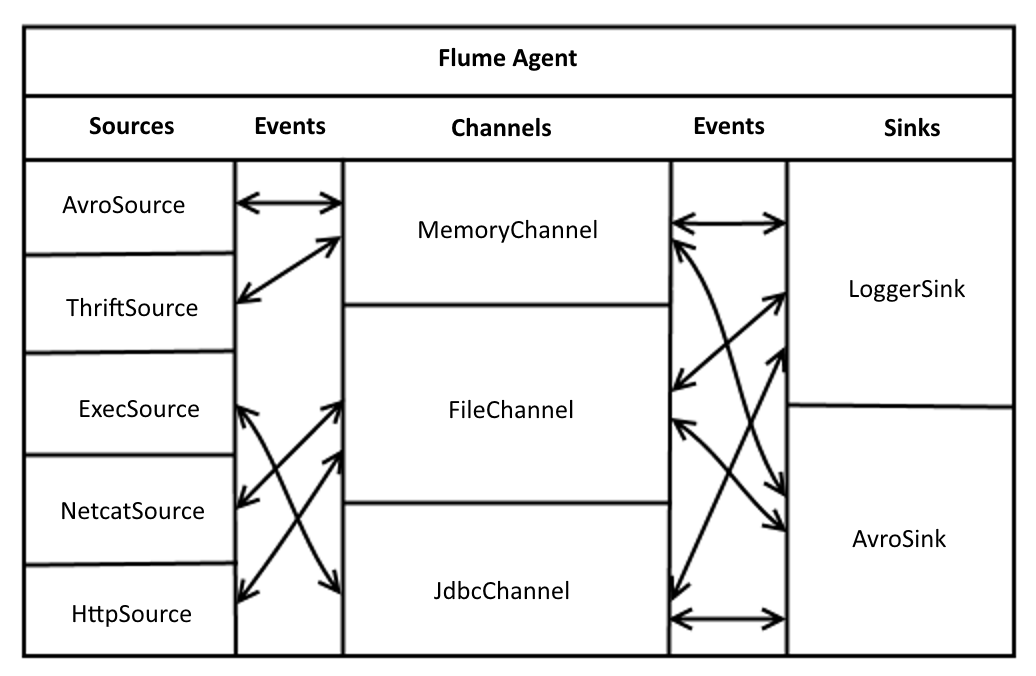
\includegraphics[width=1.0\textwidth]{bilder/flumeAgent.png}
\caption{Apache Flume Agent - Ein Agent mit mehreren Sources, Channels und Sinks
\label{fig:flumeAgent}}
\end{figure}

Ein \textit{Channel} stellt in Apache Flume einen Zwischenspeicher dar. Nachrichten werden in einem \textit{Dataflow} von der \textit{Source}, über den \textit{Channel} an den \textit{Sink} übertragen. In einem \textit{Channel} können Nachrichten in einem flüchtigen Speicher dem \textit{MemoryChannel} oder einem dauerhaften Speicher dem \textit{FileChannel} abgelegt werden. Spezifische \textit{Channel} müssen die Klasse \textit{BasicChannelSemantics} \citeint{flume:apidoc:basicChannelSemantics} erweitern oder die Klasse \textit{AbstractChannel} bei bestehenden Transaktionsmethoden erweitern. Der \textit{JdbcChannel} stellt für die Datenpersistenz über die Konfigurationsdatei eine Verbindung mit einem SQL-Server her. Der \textit{MemoryChannel} ist nicht transaktionssicher. Wenn der \textit{Agent} ausfällt gehen Nachrichten im flüchtigen Speicher verloren. Der \textit{FileChannel} schreibt im Gegensatz zum \textit{MemoryChannel} die Nachrichten in ein definiertes Verzeichnis einer Festplatte. Um die Atomarität in Apache Flume beim Persistieren einzuhalten, wird das Prinzip von \gls{glo:wal} eingesetzt. Mit dem \gls{glo:wal} wird der Eingang und der Ausgang des \textit{Channels} aufgezeichnet. Wenn der \textit{Agent} neugestartet wird, kann das \gls{glo:wal} wieder abgearbeitet werden, damit alle eingegangenen Nachrichten ausgeliefert werden. Einem \textit{Channel} kann eine Kapazität als Parameter in der Konfiguration übergeben werden. Wenn die Kapazität für die Übertragung der Nachrichten erschöpft ist, werden keine weitere Nachrichten angenommen und ein Fehler \textit{ChannelException} wird geworfen. \citelit[S. 25, Kap. 3]{flumeDistributed}

Die Ausgabe aus einem \textit{Channel} erfolgt über einen \textit{Sink}. Mit dem \textit{LoggerSink} werden Protokolldaten abhängig von der Konfiguration auf die Standardausgabe oder in eine Datei ausgegeben. Der \textit{AvroSink} \citeint{flume:apidoc:avroSink} und der \textit{ThriftSink} \citeint{flume:apidoc:thriftSink} erweitern die Klasse \textit{AbstractRpcSink} \citeint{flume:apidoc:abstractRpcSink} und ermöglichen mit deren Pendant \textit{AvroSource} und \textit{ThriftSource} \textit{Agents} miteinander zu verbinden. Ein Modell eines Datenfluss \textit{data flow} unterstützt dabei die Übersicht. Beziehungen zwischen den \textit{Agents} werden in den spezifischen Konfigurationsdateien abgelegt. In Abbildung \ref{fig:flumeAgentChaining} werden Vier \textit{Agents} dargestellt. Es wird eine Trennung des Datenstroms in \textit{Agent} 2 und eine Zusammenführung des Datenstroms in \textit{Agent} 3 gezeigt. Der Datenfluss in \textit{Agent} 2 wird durch verwenden mehrere \textit{Channels} aufgeteilt. Der Ausgabestrom \textit{Sink} A jeweils aus \textit{Agent} 1 und \textit{Agent} 2 wird in die \textit{Source} A von \textit{Agent} 3 geleitet. Und der Ausgabestrom \textit{Sink} B aus \textit{Agent2} wird in die \textit{Source} A eines separaten \textit{Agent} 4 geleitet.

\begin{figure}[htb!]
\centering
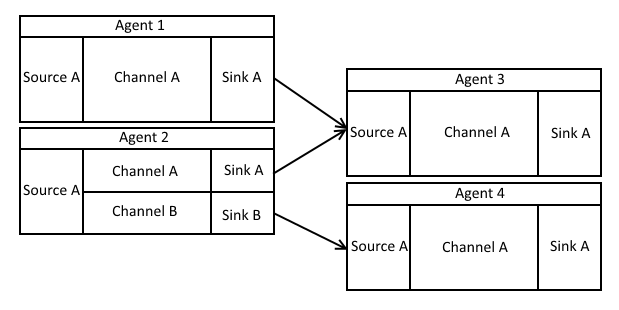
\includegraphics[width=1.0\textwidth]{bilder/flumeAgentChaining.png}
\caption{Apache Flume Agent Datenfluss
\label{fig:flumeAgentChaining}}
\end{figure}

Bei hoher Last oder einer Ausfallsicherung ist es möglich \textit{sinkgroups} einzusetzen. Eine \textit{Sinkgroup} mit dem Prozessortyp \textit{load\_balance} kann eine Last je nach Parameter per \textit{round\_robin} oder \textit{random} mehrere \textit{Sinks} gleich verteilen. In der Ausfallsicherung muss der Prozessortyp \textit{failover} verwendet werden. Den verwendeten \textit{Sinks} wird über Parameter eine Priorität zugeordnet. Nach einem Ausfall eines \textit{Agents} wird nach der Prioritätenliste der nächste verfügbare \textit{Agent} eingesetzt. \citelit[S. 43]{flumeDistributed}

In Abbildung \ref{fig:flumeAgentChaining} schreibt die \textit{Source} A vom \textit{Agent} 2 abhängig vom \textit{Flume Event} in \textit{Channel} A oder \textit{Channel} B. Über den Parameter \textit{selector} ist es möglich \textit{Flume Event} in bestimmte \textit{Channels} zu leiten. Mit dem \textit{selector}-Typ \textit{multiplexing} und dem Parameter \textit{mapping} können \textit{Flume Events} abhängig vom \textit{Header} zu einem \textit{Channel} geleitet werden. Die Standardeinstellung im Vergleich zu \textit{multiplexing} ist \textit{replicating}. Durch den \textit{selector}-Typ \textit{replicating} werden \textit{Flume Events} an alle \textit{Channels} innerhalb eines \textit{Agents} geleitet. \citelit[S. 58]{flumeDistributed}

Ein \textit{Agent} kann als Sammler \textit{collector} der \textit{Flume Events} in einem Bulk von verschiedenen \textit{Agents} aufnimmt und weiterleitet. Somit sind mit Apache Flume Schichten möglich. In der ersten Schicht können mehrere \textit{Agents} Nachrichten von \textit{Clients} aufnehmen, in \textit{Flume Events} umwandeln und in bestimmten Zeitabständen an den Sammel-\textit{Agent} weiter leiten. In der Zweiten Schicht können die Daten zur weiteren Verarbeitung an Apache Hadoop und Apache Storm oder zur Datensicherung in ein sequentiellen Speicher weiter geleitet werden. \citelit[S. 70]{flumeDistributed}

Nachrichten können während der Laufzeit mit speziellen \textit{Interceptors} verarbeitet werden. Spezifische \textit{Interceptor} müssen die Schnittstellen \textit{Interceptor} und \textit{Interceptor.Builder} implementieren. Folgende List gibt einen Überblick über die bestehenden Typen.
\begin{description}
	\item[TimestampInterceptor] setzt den aktuellen Zeitstempel im Header aller abgefangenen \textit{Flume Events} \citeint{flume:apidoc:timestampInterceptor}
	\item[HostInterceptor] fügt den Namen der Maschine oder die IP-Adresse in den \textit{Header} aller abgefangenen \textit{Flume Events} hinzu \citeint{flume:apidoc:hostInterceptor}
	\item[StaticInterceptor] fügt ein definiertes Schlüssel/Wert-Paar in den \textit{Header} aller abgefangenen \textit{Flume Events} ein \citeint{flume:apidoc:staticInterceptor}
	\item[RegexFilteringInterceptor] verwendet das Java-Paket \textit{java.util.regex} mit einem definierten Ausdruck und prüft den \textit{Body} eines \textit{Flume Events}, ob der Ausdruck passt. Mit dem Parameter \textit{excludeEvents} werden die \textit{Flume Events} für die weitere Übertragung eingeschlossen oder ausgeschlossen. \citeint{flume:apidoc:RegexFilteringInterceptor}
	\item[RegexExtractorInterceptor] setzt ebenfalls das Java-Paket \textit{java.util.regex} ein und sucht nach durch den regulären Ausdruck nach Mustern. Gefundene Muster werden als Schlüssel/Wert-Paar in den Header des \textit{Flume Events} hinzugefügt. In den Parametern \textit{serializers} muss Anzahl und der Bezeichner der Anzahl Platzhalter im regulären Ausdruck entsprechen. \citeint{flume:apidoc:RegexExtractorInterceptor}
\end{description}

Apache Flume bietet Zwei verschiedene \textit{Monitoring}-Typen \textit{Ganglia}\footnote{Ganglia Monitoring System - \url{http://ganglia.sourceforge.net/}} und \textit{Http}. Der beim Start eines \textit{Agents} verwendete Typ \textit{http}, erzeugt eine Web-Server-Instanz und bei einer Anfrage wird eine Metrik als \gls{glo:json} zurückgegeben. Die Monitoring-Anwendung Nagios kann durch aktive Prüfungen das \gls{glo:json} filtern und das Ergebnis im \textit{Service}-Bereich darstellen. Mit Ganglia-Integration können ähnlich wie in Nagios bestimmte Metriken ohne JSON zu filtern direkt abgerufen werden. Eine weitere \textit{Monitoring}-Möglichkeit besteht über \gls{glo:jmx} und der Java-Anwendung JConsole. Mit der JConsole können die die \textit{MBean}-Attribute ausgelesen werden. Alternativ ähnlich wie in Apache Kafka kann über das \gls{glo:jmx}-Plugin in Nagios eine Abfrage auf die gegebenen Attribute erfolgen. In der Liste \ref{lst:flumeMonitoring} wird ein Beispiel für das \textit{Monitoring} über \gls{glo:http} gezeigt. Die gezeigten Argumente können beim Programmaufruf oder in der Konfigurationsdatei hinzugefügt werden. \citelit[S. 77, Kap. 7]{flumeDistributed}


\begin{lstlisting}[language=BASH, label=lst:flumeMonitoring, caption=Apache Flume Monitoring]
-Dflume.monitoring.type=http
-Dflume.monitoring.port=55555
\end{lstlisting}

\begin{table}[ht!]
	\centering
		\begin{tabular}{@{}ll@{}} \toprule
			\textbf{Kriterium} & \textbf{Bewertung} \\ \midrule
			Architektur & Strukturierte Peer-to-Peer-Architektur \\
			Prozesse und Threads & Client-Server-Modell und \gls{glo:rpc} \\
			Kommunikation & Streamorientierter synchroner Übertragungsmodus \\
			Namenssystem & Hierarchische Benennung \\
			Synchronisierung & Dezentraler Algorithmus \\
			Pipelining und Materialisierung & Agent chaining \\
			Konsistenz und Replikation & Replikation und Multiplexing \\
			Fehlertoleranz & Load balancing und Failover \\ 
			Sicherheit & Verschlüsselung und Datenkompression mit Apache Avro, \\			
			& HTTPSource unterstützt SSL, \\
			& Monitoring mit JMX, Ganglia und Nagios\\
			Erweiterung & Eigenentwicklung und Community-Beiträge \\
			Qualität & FileChannel \gls{glo:wal} \\
			\bottomrule			
		\end{tabular}
	\caption{Bewertung Apache Flume}
	\label{tab:bewflume}
\end{table}

In diesem Kapitel und im Anhang wurde gezeigt wie Apache Flume installiert und für eine einfache Client/Server-Anwendung konfiguriert werden kann. Es wurden Techniken gezeigt, um Daten zu aggregieren, weiter zu leiten und zur Laufzeit zu bearbeiten. Verschiedene Einstiegspunkte im Quelltext von Apache Flume wurden gegeben, um spezifische Implementierungen zu entwickeln. Zuletzt wurden verschiedene Software-Werkzeuge für das \textit{Monitoring} gezeigt. Im nächsten Kapitel wird Apache S4 vorgestellt.

%Instead of focusing on analytics, Flume focuses primarily upon data transport and integration with a wide set of data sources and data destinations.
%http://www.ibm.com/developerworks/opensource/library/bd-flumews/index.html
%http://blog.cloudera.com/blog/2013/01/how-to-do-apache-flume-performance-tuning-part-1/
%\citelit{rfc4422}